% ----------------------------------------------------------
% VERSÃO ORIGINAL
% ----------------------------------------------------------
% The Current Maintainer of this work is the abnTeX2 team, led
% by Lauro César Araujo. Further information are available on
% http://abntex2.googlecode.com/

\documentclass[
	% -- opções da classe memoir --
	12pt,				% tamanho da fonte
	openright,			% capítulos começam em pág ímpar (insere página vazia caso preciso)
	oneside,			% para impressão em verso e anverso coloque twoside
	a4paper,			% tamanho do papel.
	% -- opções da classe abntex2 --
	%chapter=TITLE,		% títulos de capítulos convertidos em letras maiúsculas
	%section=TITLE,		% títulos de seções convertidos em letras maiúsculas
	%subsection=TITLE,	% títulos de subseções convertidos em letras maiúsculas
	%subsubsection=TITLE,% títulos de subsubseções convertidos em letras maiúsculas
	% -- opções do pacote babel --
	french,				% idioma adicional para hifenização
	spanish,			% idioma adicional para hifenização
	english,			% idioma adicional para hifenização
	brazil				% o último idioma é o principal do documento
	]{abntex2}


% ----------------------------------------------------------
% PACOTES
% ----------------------------------------------------------
% ----------------------------------------------------------
% PACOTES BÁSICOS
% ----------------------------------------------------------
\usepackage{lmodern}            % Usa a fonte Latin Modern          
\usepackage[T1]{fontenc}        % Selecao de codigos de fonte.
\usepackage[utf8]{inputenc}     % Codificacao do documento (conversão automática dos acentos)
\usepackage{lastpage}           % Usado pela Ficha catalográfica
\usepackage{indentfirst}        % Indenta o primeiro parágrafo de cada seção.
\usepackage{color}              % Controle das cores
\usepackage{graphicx}           % Inclusão de gráficos
\usepackage{microtype}          % para melhorias de justificação
\usepackage{listings}           % Inserir código de linguagem de programação
\usepackage{nomencl}            % Necessário para o commando makeindex
\usepackage{textcomp}
 \usepackage{float}
% Pacotes de citações
\usepackage[brazilian,hyperpageref]{backref}     % Paginas com as citações na bibl
\usepackage[alf]{abntex2cite}   % Citações padrão ABNT

% CONFIGURAÇÕES DE PACOTES
% Configurações do pacote backref
% Usado sem a opção hyperpageref de backref
\renewcommand{\backrefpagesname}{Citado na(s) página(s):~}
% Texto padrão antes do número das páginas
\renewcommand{\backref}{}
% Define os textos da citação
\renewcommand*{\backrefalt}[4]{
    \ifcase #1 %
        \relax%
    \or
        Citado na página #2.%
    \else
        Citado #1 vezes nas páginas #2.%
    \fi}%

% ----------------------------------------------------------
% CAPA E FOLHA DE ROSTO
% ----------------------------------------------------------
% ----------------------------------------------------------
% CAPA E FOLHA DE ROSTO
% ----------------------------------------------------------
\titulo{Sobre a Termodinâmica planetária}
\autor{Saulo Fernandes Benquerer}
\local{Uberlândia}
\data{Junho de 2025}
\tipotrabalho{Tese (Graduação)}
\preambulo{Tese de Física de autoria de Saulo Benquerer Nome de batismo: Lorena Fernandes Costa }

% ----------------------------------------------------------
% CONFIGURAÇÕES
% ----------------------------------------------------------

% Configurações de aparência do PDF final

% alterando o aspecto da cor azul
\definecolor{blue}{RGB}{41,5,195}

% informações do PDF
\makeatletter
\hypersetup{
        %pagebackref=true,
        pdftitle={\@title},
        pdfauthor={\@author},
        pdfsubject={\imprimirpreambulo},
        pdfcreator={LaTeX with abnTeX2},
        pdfkeywords={abnt}{latex}{abntex}{abntex2}{trabalho acadêmico},
        colorlinks=true,            % false: boxed links; true: colored links
        linkcolor=black,             % color of internal links
        citecolor=black,             % color of links to bibliography
        filecolor=magenta,              % color of file links
        urlcolor=black,
        bookmarksdepth=4
}
\makeatother

% Espaçamentos entre linhas e parágrafos
% O tamanho do parágrafo é dado por:
\setlength{\parindent}{1.3cm}

% Controle do espaçamento entre um parágrafo e outro:
\setlength{\parskip}{0.2cm}  % tente também \onelineskip

% compila o indice
\makeindex
\makenomenclature

% ----------------------------------------------------------
% INÍCIO DOCUMENTO
% ----------------------------------------------------------
\begin{document}

% Retira espaço extra obsoleto entre as frases.
\frenchspacing

% ----------------------------------------------------------
% ELEMENTOS PRÉ-TEXTUAIS
% ----------------------------------------------------------
% \pretextual

% Capa
\imprimircapa

% Folha de rosto
% (o * indica que haverá a ficha bibliográfica)
\imprimirfolhaderosto*

% ----------------------------------------------------------
% AGRADECIMENTOS
% ----------------------------------------------------------
\begin{agradecimentos}

Esse trabalho é fruto de todo amor que já recebi. 
\par
Seria impossível citar todas as pessoas que me ajudaram a torná-lo possível então agradeço à todas as pessoas que já me ofereceram uma palavra amiga ao longo da vida. 
Agradeço à todos os professores que incentivaram meu pensamento crítico, principalmente meu primeiro professor: meu pai. Somente minha família sabe a dor da ausência dele, e à minha família agradeço ao suporte que recebi ao longo dos anos. 

\end{agradecimentos}
% ----------------------------------------------------------
% RESUMOS
% ----------------------------------------------------------

% resumo em português
\setlength{\absparsep}{18pt} % ajusta o espaçamento dos parágrafos do resumo
\begin{resumo}

A Crise Climática gera bastante angústia ao redor do mundo e, mesmo que a sociedade pense que a culpa é da queima de combustíveis fósseis, ainda é difícil pensar em uma sociedade que não utilize petróleo. No entendimento atual, o dióxido de carbono(CO2) é o principal culpado do aumento do Efeito Estufa que gera o Aquecimento Global. Essa tese é contrária a visão das Mudanças Climáticas atual e coloca os sistemas de Ar-Condicionados como culpados.
\par
Primeiro será explicado as razões para essa mudança de perspectiva e será proposto um experimento para confirmar ou negar essa tese, e em seguida, trabalhos futuros envolvendo o uso de um novo sistema de refrigeração

    \vspace{\onelineskip}
    \noindent 
    \textbf{Palavras-chaves}: Aquecimento Global, Crise Climática, Efeito Estufa, Ar-condicionados, Refrigeração Geotérmica
\end{resumo}

% resumo em inglês
\begin{resumo}[Abstract]
 \begin{otherlanguage*}{english}

The Climate Crisis generates a lot of distress around the world and even as the scientific consensus thinks that the use of fossil fuel is the culprit - it's still hard to imagine a world without the use of oil. The current understanding is that carbon dioxide (CO2) increases the Greenhouse Effect that in turn generates the Global Warming. This thesis opposes this current notion of the Climate Change and blames the air conditioning systems.
\par
The rationale behind this change of perspective will be explained in the beginning and then a new experiment to prove the hypothesis will be proposed. Finally, future work will be suggested involving a new refrigeration system.

    \vspace{\onelineskip}
    \noindent 
    \textbf{Key-words}: Global Warming, Climate Crisis ,Greenhouse Effect, Air Conditioning, Geothermal Refrigerator
 \end{otherlanguage*}
\end{resumo}


% ----------------------------------------------------------
% inserir lista de ilustrações
% ----------------------------------------------------------
 \pdfbookmark[0]{\listfigurename}{lof}
 \listoffigures*
 \cleardoublepage

% ----------------------------------------------------------
% inserir o sumario
% ----------------------------------------------------------
 \pdfbookmark[0]{\contentsname}{toc}
 \tableofcontents*
 \cleardoublepage

% ----------------------------------------------------------
% ELEMENTOS TEXTUAIS
% ----------------------------------------------------------
\textual

\chapter*[Introdução]{Introdução}
\addcontentsline{toc}{chapter}{Introdução}

As mudanças climáticas são um dos principais campos de estudos nas últimas décadas, causando grande preocupação dentro e fora do meio científico. A príncipio foi descoberta a sua relação com a queima de combustível fóssil que incrementa o Efeito Estufa em um processo que foi denominado \textit{Aquecimento Global}. Porém, logo percebeu-se que o planeta não estava aquecendo de forma uniforme; inclusive com invernos mais rigorosos em alguns locais. Por isso, o fenômeno foi renomenado para \textit{Mudanças Climáticas} ou \textit{Crise Climática}.

A disparidade das previsões de cientistas climáticos com a realidade tem sido percebida pela sociedade ao longo dos últimos anos, o que gera angústia social e paralisia; por não sabermos como melhor atuar para resolver o problema. Esta incerteza nas previsões metereológicas atrapalham na agricultura e em outros setores da economia. Além de já ter causado mortes e colocado vidas em risco devido à problemas como enchentes, alagamentos, estiagens e outros eventos catastróficos. 

Essa tese tem como por objetivo fornecer um melhor entendimento sobre a termodinâmica da atmosfera terrestre, bem como sugerir tecnologias para estabilizar o clima e mitigar possíveis eventos climáticos extremos do futuro. A princípio, o foco é no entendimento do equívoco em colocar a queima de combustíveis fósseis como protagonista nas catrástofes climáticas que têm ocorrido ao redor do mundo. Em seguida serão apresentadas as ferramentas para eliminar os eventos climáticos extremos e, por consequência, obter uma maior estabilidade climática. Por fim, serão apresentados possíveis trabalhos futuros e campos de estudo para aprofundar o conhecimento do funcionamento climático global.
\cleardoublepage
%\part*{Desenvolvimento}
\chapter[Ar-condicionados]{Ar-condicionados}

A termodinâmica ganhou bastante destaque desde a revolução industrial, pois seu estudo contribuiu para criação e melhoria de diferentes máquinas térmicas - principalmente máquinas a vapor - e continua tendo bastante importância no mundo moderno. Toda tecnologia que está em nossa volta teve contribuição da ciência da termodinâmica para sua criação. Por isso, mesmo que a sociedade considera as mudanças climáticas como consequência dessas tecnologias, não queremos parar de utilizá-las.

Existe uma transferência natural de energia entre corpos quentes para corpos mais frios - este fenômeno é denomidado calor. A tranferência de calor pode ocorrer por três meios distintos: radiação, convecção e condução - e se dois corpos já nâo trocam mais calor considera-se que estão em equilíbrio térmico. A troca de calor entre dois ou mais corpos podem afetar outras propriedades além da temperatura, tais como o volume e a pressão; e o ramo da física que estuda esses efeitos é a Termodinâmica \cite{Maxwell}.

O calor segue o fluxo de corpos de temperatura mais alta para os de mais baixa - fato conhecido como Segunda Lei da Termodinâmica - portanto máquinas que forçam o calor a seguir o caminho oposto ao natural, tais como geladeiras e ar-condicionados, geram sempre um custo. As máquinas térmicas em fluxo inverso (refrigeradores) foram inicialmente pensados como uma forma de calcular o rendimento máximo possível de motores térmicos por Sadi Carnot \cite{Carnot}. Porém, ar-condicionados acabaram sendo construídos sem que o seu custo em termos de aumento da entropia atmosférica fosse devidamente levado em consideração.

A analogia feita por Sadi Carnot foi comparar máquinas térmicas à uma cachoeira - sendo a fonte quente como o topo da cachoeira e a fonte fria em baixo. Desta forma é possível ver o absurdo que é querer forçar o calor a seguir um fluxo contrário ao seu natural. Por mais que seja possível fazer isso com pequenas quantidades de energia, em larga escala a cachoeira jamais irá subir com sua água. E na prática, não existe um isolamento forte entre a Fonte Quente e a Fria no caso de ar-condicionados, o que faz com que tenha um grande disperdício de energia (\autoref{carnot}).

\begin{figure}[h]
    \centering
    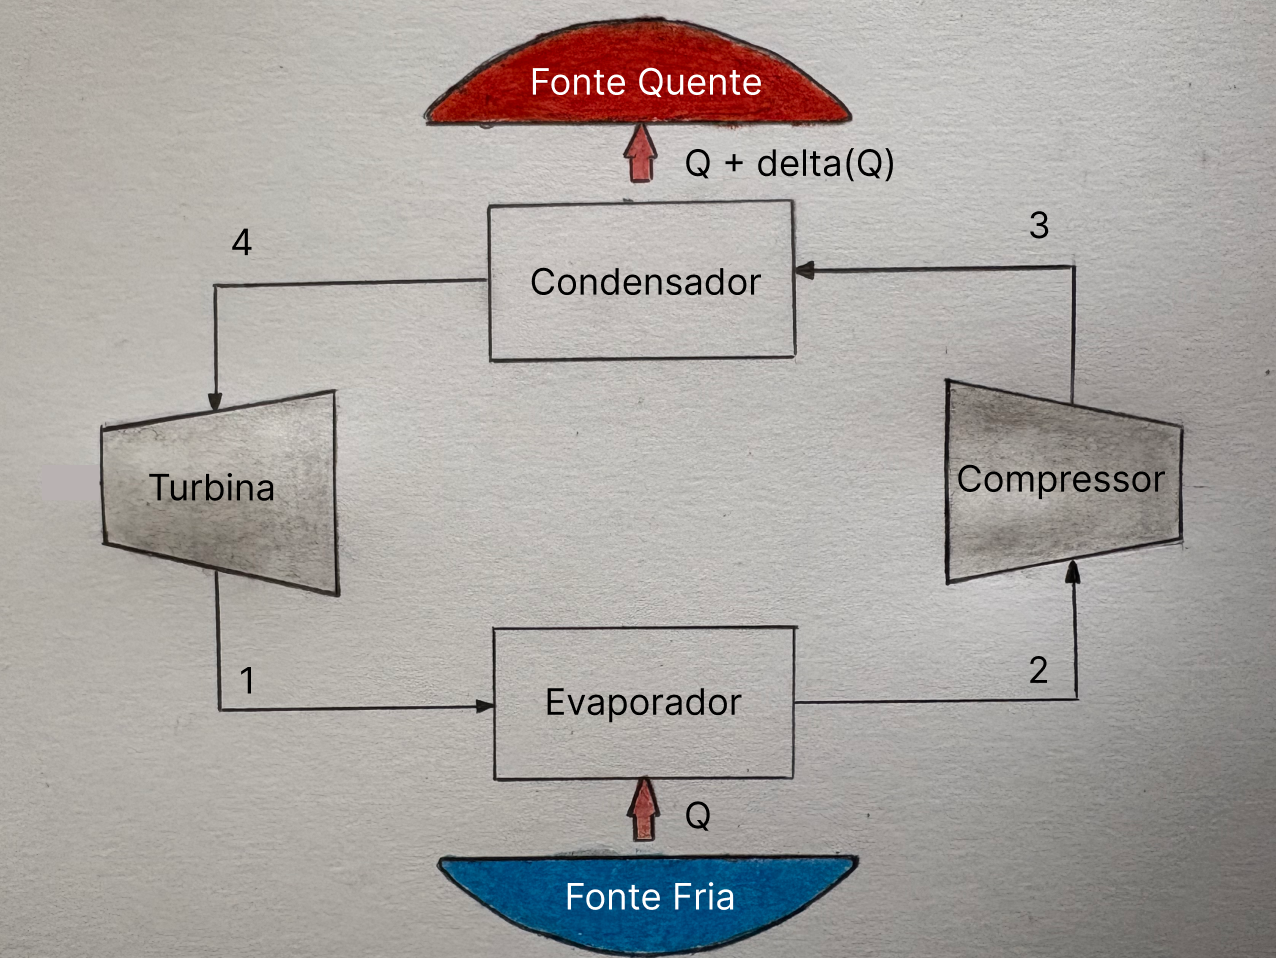
\includegraphics[scale=0.25]{pictures/carnot.png}
    \caption{Esquema do ciclo reverso de Carnot - considerado um refrigerador ideal e impossível na prática.}
    \label{carnot}
\end{figure}

Em outras palavras, ar-condicionados afetam de forma intensa a entropia da atmosfera, definido por Rudolf Clausius como a variação infinitesimal da quantidade calor pela temperatura instântanea. A entropia as vezes é denominada como medida do caos de um sistema, ou seja, se queremos estabilidade climática é essencial estar atento a máquinas que aumentam essa propriedade de forma intensa \cite{Clausius}.

O sistema de ar-condicionado simplesmente joga o calor de um cômodo para o exterior, e nesse processo parte da energia elétrica empregada é convertida em mais energia térmica. Como o calor segue seu fluxo natural, durante o período de funcionamento do ar-condicionado parte da energia térmica volta para o cômodo de origem. Além disso, como o ar quente tende a subir, o efeito é pior em casos de ACs(ar-condicionados) de andares inferiores de prédio, pois o calor eliminado irá para os apartamentos vizinhos. Nos centros urbanos estamos desperdiçando energia ao usar os ACs como método de refrigeração.

\begin{figure}[h]
    \centering
    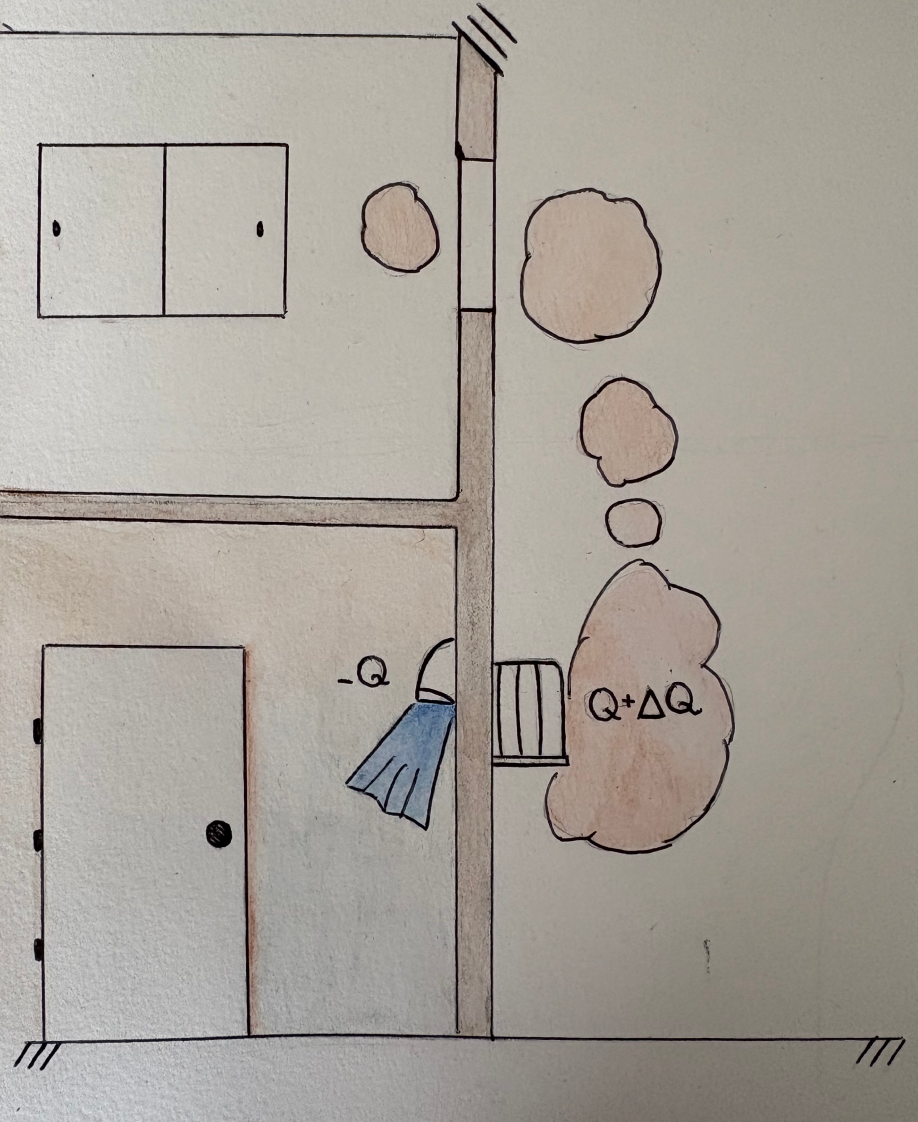
\includegraphics[scale=0.35]{pictures/predio.png}
    \caption{Ilustração do funcionamento do ar-condicionado - aumentando o calor e retornando para o ambiente de origem e apartamentos vizinhos.}
    \label{carnot}
\end{figure}

Uma analogia para o ar-condicionado é alguém retirando água com balde de um navio furado, não resolve o problema e possui um alto gasto energético, pois a água prontamente tenta retornar ao barco. Os ACs são geladeiras com portas abertas: podem aliviar o problema do calor para a pessoa imediatamente à frente, porém quando se analisa o sistema completo, sua eficiência é negativa.\textbf{ Além do mais, o Aquecimento Global é um problema público, sua solução também precisa estar na esfera da infraestrutura pública.}
                                  
Carnot em seu tratado "Reflexões sobre energia motora e fogo" tratou as máquinas térmicas de forma relativamente isolada com o ambiente. Este é um erro bem compreensível, pois na época não era possível prever que as máquinas térmicas reversas - ar-condicionado e geladeiras - seriam utilizadas em larga escala. Porém, quando deixa de analisar as máquinas de forma isolada ao ambiente, começa a se entender o problema que culminou nas mudanças climáticas que assombram a sociedade hoje em dia.                                                         

Quando se olha para uma escala global, o efeito do ar-condicionado na atmosfera é de gerar energia térmica e aumentar a entropia da atmosfera local - gerando uma zona de alta pressão - que são as ilhas de calor urbanas (\autoref{ilha-calor}). Estas máquinas não são um regriferadores de cômodos, mas sim aquecedores do mundo. A alta pressão da ilha de calor expulsa nuvens e dificulta a precipitação de chuva. Pois o ar quente precisa de mais vapor d'água para que ocorra a chuva que realmente resfriaria o ambiente urbano. Por isso, quando chove a quantidade de água é mais elevada causando tempestades, ciclones-bomba e enchentes. 

\begin{figure}[h]
    \centering
    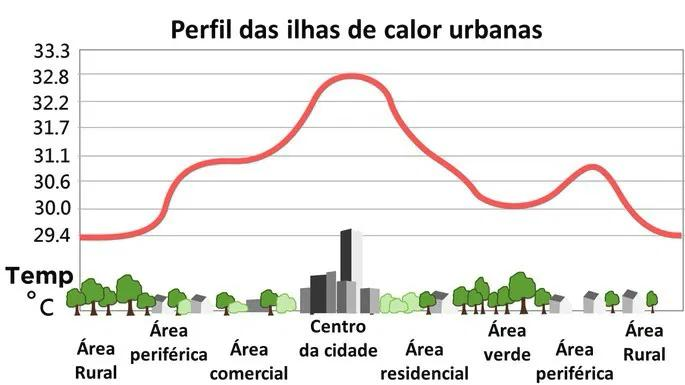
\includegraphics[scale=0.6]{pictures/ilha-calor.jpg}
    \caption{Ilustração da ilha de calor gerada pela alta queima de conbustível fóssil e refrigeração ineficiente.}
    \label{ilha-calor}
    \legend{Fonte: https://www.todamateria.com.br/ilha-de-calor/}
\end{figure}

Considerar a atmosfera como reservatório térmico com capacidade infinita é o erro que provocou o uso em larga escala do ar-condicionado. Apesar de ser verídico que a atmosfera terrestre possui grande capacidade térmica quando comparado a objetos humanos do dia-a-dia. Quando analisamos a sociedade como todo percebemos que máquinas térmicas são capazes de afetar a atmosfera em grande escala, pois estamos lidando em uma escala de centenas de milhões de ar-condicionados ao redor do mundo; e muitos deles bem concentrados em bairros específicos. 
Além disso, o ar-condicionado perde eficiência quando a temperatura externa está alta, ou seja, quando mais as pessoas têm o ímpeto de utilizar essa máquina - que são os dias quentes - menos eficiente estas serão em seu "trabalho".

                                        
\chapter[Efeito Estufa]{Efeito Estufa}

O efeito estufa é o processo de reabsorção dos raios infravermelhos pela atmosfera e é essencial para a vida, pois se este não existisse, o planeta seria muito mais frio: por volta de -18°C \cite{Nasa-cold}. O problema com a forma atual de estudar esse fenõmeno é que estamos tentando dissecar a contribuição dos diversos componentes da atmosfera e estudá-los separadamente.

O que chamamos de efeito estufa é a resistência gerada pela pressão radioativa solar em contraponto com a radiação refletida pela superfície do planeta. Sabemos que a radiação emitida por uma estrela decresce com o quadrado da distância. A temperatura máxima que a Terra pode atingir depende muito mais da intensidade de radiação solar recebida pela posição que ocupamos no cosmos do que com a composição da atmosfera em si. Pois a posição de um planeta em relação a sua estrela não apenas afeta a quantidade de energia recebida, mas também influencia a taxa em que este perde calor para o espaço sideral. Pois não existe vácuo perfeito então a temperatura do espaço sideral em volta de um planeta também é diretamente influenciado pela distância em que ele está dessa \cite{cosmic-wave}.

Em outras palavras, apesar do efeito estufa ter grande influência no clima global, existe um limite para seu efeito de aquecimento. O Efeito Estufa é como um cobertor:  diminui a taxa de perda de calor, porém é incapaz de realmente gerar um aquecimento. Existe uma temperatura máxima que a Terra pode atingir que é influenciada pela posição da Terra em relação ao Sol e a intensidade da radiação enviada por este. Esses dois fatores mudam apenas em escalas de tempo cósmicas, sendo portanto possível estabilizar o clima do planeta à longo prazo.

Os pólos recebem uma menor incidência de raios solares e, devido ao gelo, refletem também uma parte deles,  potencializando o resfriamento do local. Com isso, existe um fluxo de calor constante entre o Equador e os pólos. A todo momento o planeta reflete parte do calor como energia luminosa para o espaço sideral. Por isso quando o Voyager tirou a sua última foto, o planeta pode ser visto como o "Pale Blue Dot", se a Terra não irradiasse energia a todo momento para o cosmos, nosso planeta não poderia ser visto.

\begin{figure}[h]
    \centering
    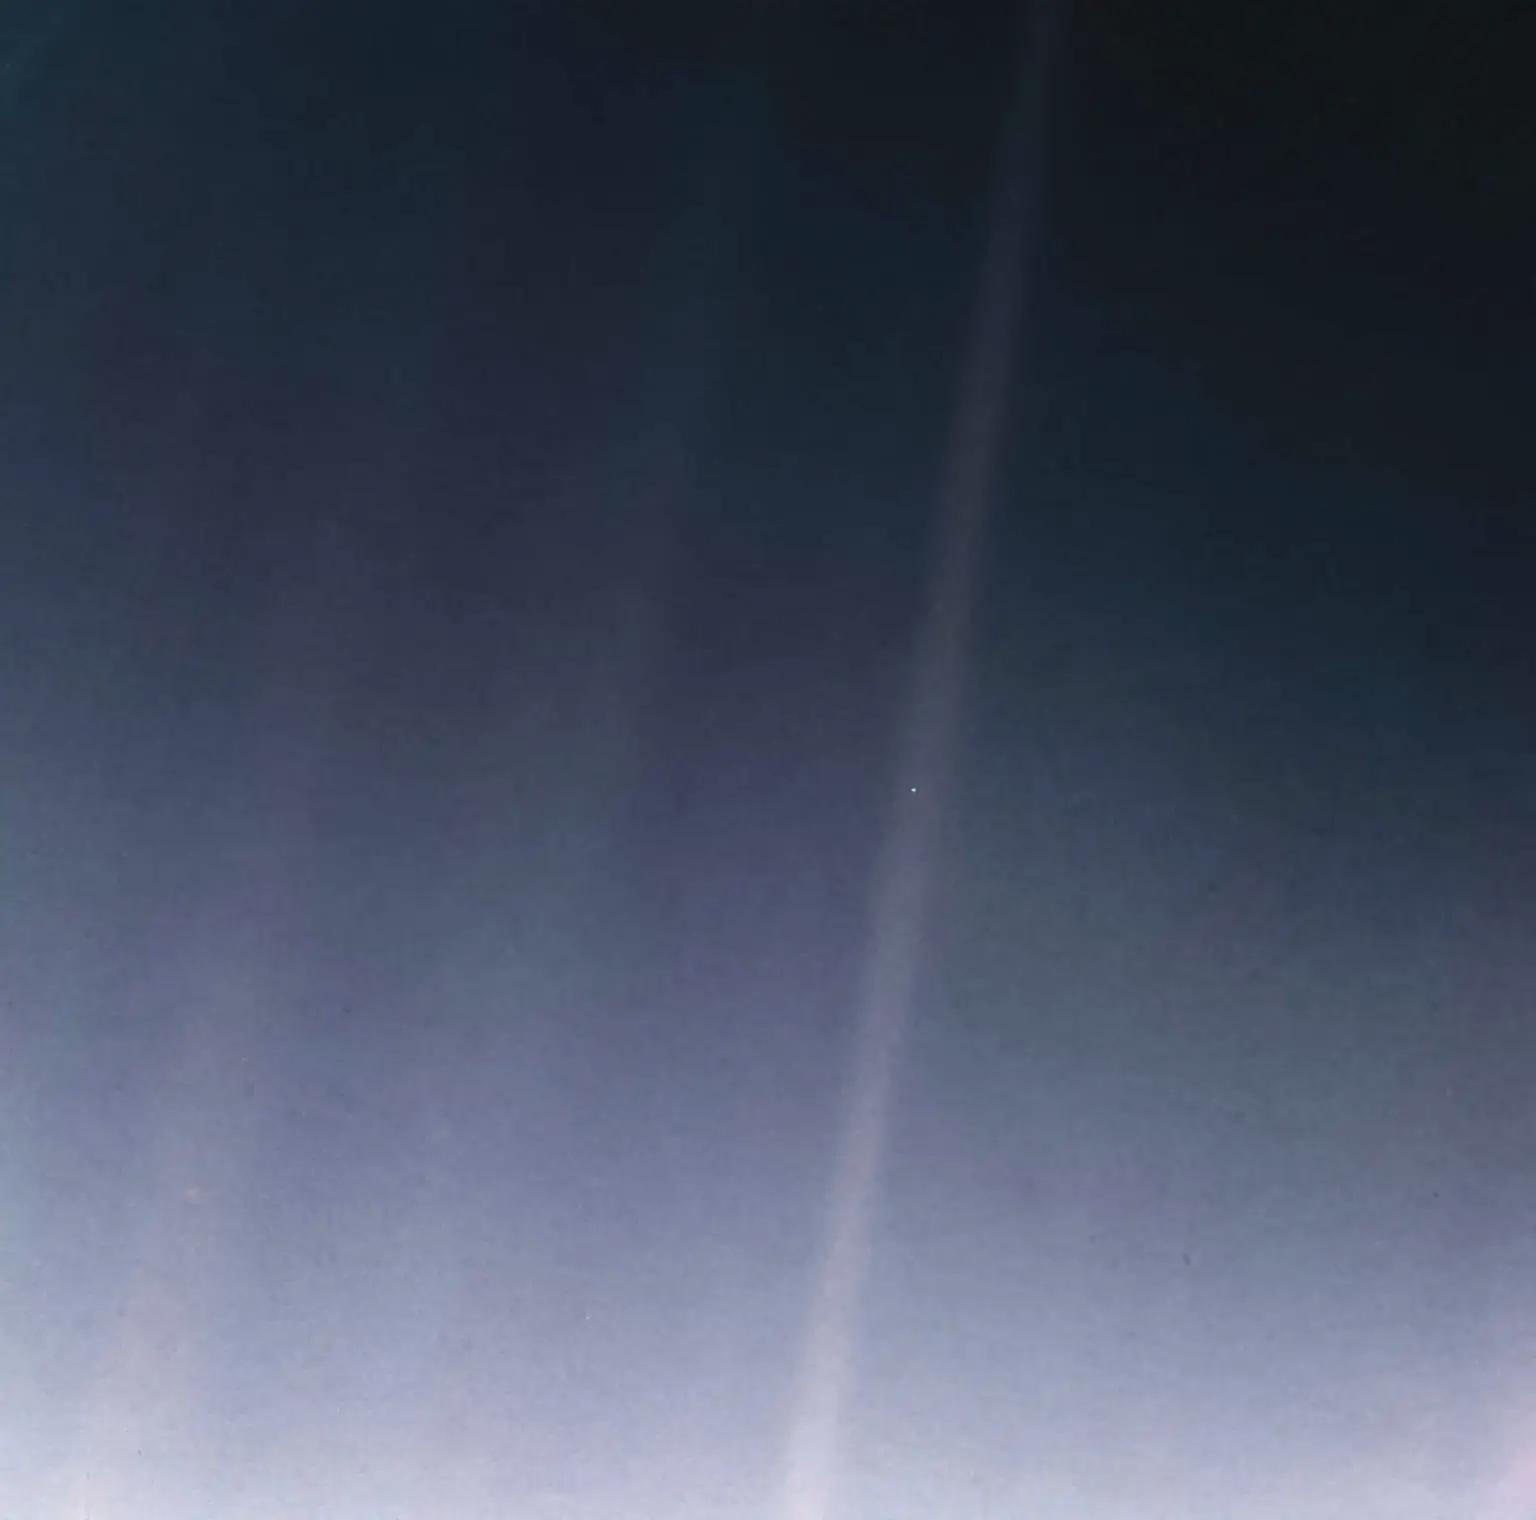
\includegraphics[scale=0.25]{pictures/pale-blue-dot.jpg}
    \caption{Imagem da Terra retirada pelo Voyager 1}
    \label{geothermal-default}
    \legend{Fonte: NASA/JPL-Caltech}
\end{figure}

Obviamente essa é uma visão simplificada da questão, pois o gelo intensifica o grau de reflexão dos raios solares e pode chegar até um ponto crítico em que gera as Eras do Gelo. Outra razão para não fazer sentido dissecar o grau de efeito estufa de cada componente atmosférico é por que dependendo da concentração o seu efeito pode inverter. Dias muito nublados e/ou com muita fumaça atmosférica faz com que mais raios solares sejam refletidos pela atmosfera do que reabsorvidos pelo Efeito Estufa, ou seja, os mesmos componentes podem afetar o clima de forma diferente em circunstâncias diversas.

Além disso, devido a rotação do planeta existe a diferença entre dia e noite em lados opostos da Terra, essa diferença também influencia os ventos terrestres. Pois durante a noite o planeta perde energia térmica de forma mais intensa para o cosmos, o que acaba trazendo ventos das áreas mais aquecidas para essas regiões devido ao fluxo natural do calor.

O mais famoso gás do efeito estufa é o dióxido de carbono, que é produzido principalmente pela queima de combustíveis fósseis tais como petróleo ou carvão. Porém, existe outros gases que possuem essa propriedade, tais como o metano - que gera bastante discussão em termos do efeito da agropecuária nas mudanças climáticas. 
As plantas absorvem dioxido de carbono para produzir matéria orgânica e muitas evoluiram no período Carbonífero onde a concentração de CO2 era bem mais alta, ou seja, as emissões desse gás vão somente potencializar o efeito de crescimento das plantas se a humanidade não continuar com práticas abusivas de desmatamento.

Apesar de menos discutido o vapor d'água tem propriedades de efeito estufa que funcionam como uma retroalimentação ou também chamado de efeito \textit{feedback} \cite{Soden}. Este nome é dado por que quanto mais quente estiver, mais vapor d'agua pode ficar retido sem que tenha saturação ou precipitação na forma de chuva. Assim, nas ilhas de calor urbanas é possível a retenção de uma grande quantidade de água sem que haja chuva; e esse vapor d'agua vai potencializar a sensação térmica no ambiente devido a sua capacidade de efeito estufa.

Porém, mesmo que todo combustível fóssil seja consumido, a temperatura da Terra ainda estaria em um patamar agradável para a vida, como já ocorreu em outros períodos geológicos. A temperatura mínima e máxima que um planeta pode atingir depende principalmente da distância que este está da estrela em que orbita e o tipo dessa estrela. Portanto, Vênus sempre será muito quente para a vida como conhecemos e Marte não recebe energia solar o suficiente para sustentá-la - sem que se contrua alguma usina nuclear o que parece algo improvável em um futuro próximo. O foco de cientistas ambientais deve ser portanto em controlar os níveis de entropia da atmosfera: primeiro parando com o uso dos ar-condicionados e depois criando sistemas de refrigeração geotérmica.

Além disso, é um erro pensar que o aumento da temperatura na Terra vai causar um aumento no nível dos oceanos de forma direta. O aumento da temperatura irá influenciar o ciclo da água, formando mais tempestades que por sua vez poderão aumentar rios e lagos, que podem ser direcionadas para regiões áridas com o uso da refrigeração geotérmica.

\section{Ilhas de calor e Rio Grande do Sul}

As ilhas de calor formadas pelas metrópoles do Sudeste que possuem uma alta concentração de ar-condicionados fazem com que se tenha uma dificuldade na saturação do vapor d'agua. Em outras palavras a atmosfera na região das metrópoles acaba tendo uma grande concentração de água em dias quentes, que não precipita com facilidade devido ao uso intensivo de ar-condicionado e grande quantidade de queima de combustível fóssil - muitos automóveis em um pequeno espaço. Lembrando do que já foi explicado anteriormente que a água tem um efeito de feedback em relação ao efeito estufa, exceto em caso de dias muito nublados.

Essa massa de ar com alta saturação de água segue o fluxo natural do calor, ou seja, ela segue em direção ao pólo Sul onde encontra uma frente fria que força sua saturação e por isso gera os alagamentos e enchentes que estão sendo sentidos na Região Sul do Brasil. As catastrófes vistas na Região Sul podem voltar a ocorrer se não houver uma mudança na forma que a região Sudeste se refrigera. Porém, se a refrigeração geotérmica começar a ser usada em escala, além de evitar essas tragédias, poderemos ver efeitos positivos em relação ao combate da desertificação no sertão nordestino. Os problemas opostos entre o Nordeste e Sul do país estão ambos conectados à alta entropia atmosférica das regiões metropolitanas.
\chapter[Refrigeração Geotérmica]{Refrigeração Geotérmica}

Para ter uma refrigeração real e dar conforto térmico para a população é necessário seguir as Leis da Natureza, no caso, transferir a energia térmica retirada de um ambiente para uma reservatório térmico mais frio. Na prática, o espaço sideral é a única fonte fria quando se analisa a termodinâmica em escalas planetárias. Pois o interior dos planetas têm temperaturas elevadas devido ao efeito da pressão gravitacional \cite{Simon–Glatzel}; e recebemos energia térmica do Sol durante o dia - cuja uma parte fica retida na atmosfera pelo Efeito Estufa. Porém, como o planeta perde energia térmica a todo tempo para o espaço, existe sempre uma fonte fria no subsolo (\autoref{soil-temp}). Em outras palavras, em certa profundidade do solo costuma estar em uma temperatura inferior do que na superfície durante o dia.

\begin{table}[h]
\centering
\ABNTEXfontereduzida
\caption{Temperatura do solo vs Profundidade}
\legend{Fonte: https://renouvelable-habitat.fr/en/soil-temperature-at-2m-depth}
\label{soil-temp}
\begin{tabular}{ccc}
\hline
Profundidade(m)  &    Temperatura(°C)\\
\hline
0.5 & 10 – 15 \\
1 & 12 – 15 \\
2 & 13 – 16 \\
3 & 14 – 16 \\
4 & 15 – 17 \\
5 & 15 – 18 \\
10 & 18 – 25 \\
300 & 25 – 30 \\
1000 & 30 – 50 \\
\hline
\end{tabular}
\end{table}

A refrigeração geotérmica é naturalmente mais eficiente que um ar-condicionado, pois segue o fluxo natural do calor. Existem diversas formas de projetar um refrigerador geotérmico, mas o príncipio de todos é igual: enterrar algum fluido alguns metros abaixo do solo e utilizar um sistema de bombeamento atrelado a algum radiador térmico. Usar água como fluído é a opção mais natural devido a sua ótima capacidade térmica e o fato de ser abundante na Terra.

A temperatura do solo varia de acordo com a latitude no planeta, tipo de solo, estação do ano e hora do dia, além de muitos outros fatores. Portanto, a profundidade dos poços para refrigeração geotérmica é um dado que deve ser obtido experimentalmente e não posso nessa tese estimar a quantidade de calor que pode ser retirada do ambiente usando essa tecnologia.

Porém, outra vantagem da refrigeração geotérmica, em comparação com ar-condicionados, é o fato que ela pode ser utilizada ao ar-livre. Como essa tecnologia realmente tem poder de refrigerar um ambiente - por seguir o fluxo natural do calor - o efeito do seu uso é benéfico em toda a vizinhança. Diferentemente dos ACs que pioram a qualidade térmica nos espaços vizinhos ao seu uso.

É de conhecimento público que árvores afetam positivamente o clima no local, amenizando o calor e, em muitos casos, fazendo com que a sensação térmica seja de alguns graus a menos do que na mesma cidade em um local menos arborizado. Porém, muitas vezes essa diferença é atribuída ao fato de que árvores fazem sombra, ao invés da razão principal, que é de que são capazes de puxar água que está armazenada no subsolo e que está a uma temperatura bem inferior a da atmosfera no momento. O objetivo da refrigeração geotérmica é criar o mesmo efeito de refrigeração que a arborização gera, porém sem a necessidade de esperar o crescimento da árvore. Além do fato que muitos ambientes que precisam de refrigeração não podem ter árvores no local. 

Para equacionar a termodinâmica planetária é necessário dividir entre orgânicos e inorgânicos por que os seres vivos possuem metabolismo próprio que influencia o clima global. E a vida não está distribuída igualmente entre o planeta; existe muito mais metabolismo dentro da Amazônica do que comparado ao deserto do Saara. 
De forma similar, as máquinas térmicas não se distribuem de forma igual no planeta, centros urbanos como São Paulo possuem muito mais maquinários utilizando energia do que em um vilarejo na África. Todos esses parâmetros ainda devem ser estudados com mais profundidade, e ainda deve se ter em mente que existe uma barreira de ventos entre os hemisférios terrestres, e portanto pode ser necessário medidas distintas entre eles.

A construção mais típica de refrigeradores geotérmicos consiste em enterrar tubulações com água ou outros fluídos refrigerantes, como na (\autoref{geothermal-default}). Porém, creio que esse seja um projeto ineficiente comparado a criação de poços impermeáveis conectados a um sistema de bombeamento que criará um "sistema circulátorio urbano", (\autoref{geothermal-new}). A razão é simples, quando menos terra precisar retirar para a construção mais barato fica e a quantidade de água armazenada determina o poder de refrigeração daquele refrigerador geotérmico. Este é um sistema fechado, isto é, a água que será adicionada ao poço não saíra do sistema exceto em caso de vazamento e danos.
O poço é então conectado por tubulações para múltiplos radiadores térmicos para que assim seja trocado calor com o ambiente. 

\begin{figure}[ht]
    \centering
    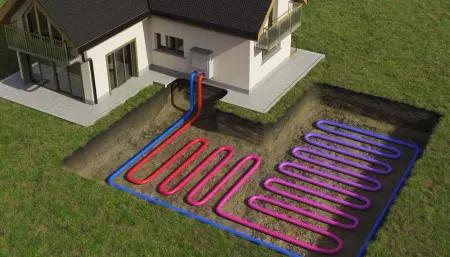
\includegraphics[scale=0.7]{pictures/geoterma-padrao.jpeg}
    \caption{Esquema de construção de geoterma com tubulação enterrada}
    \label{geothermal-default}
    \legend{Fonte: https://pt.solar-energia.net/energia-renovavel/energia-geotermica, acesso em Junho de 2025}
\end{figure}

\begin{figure}[ht]
    \centering
    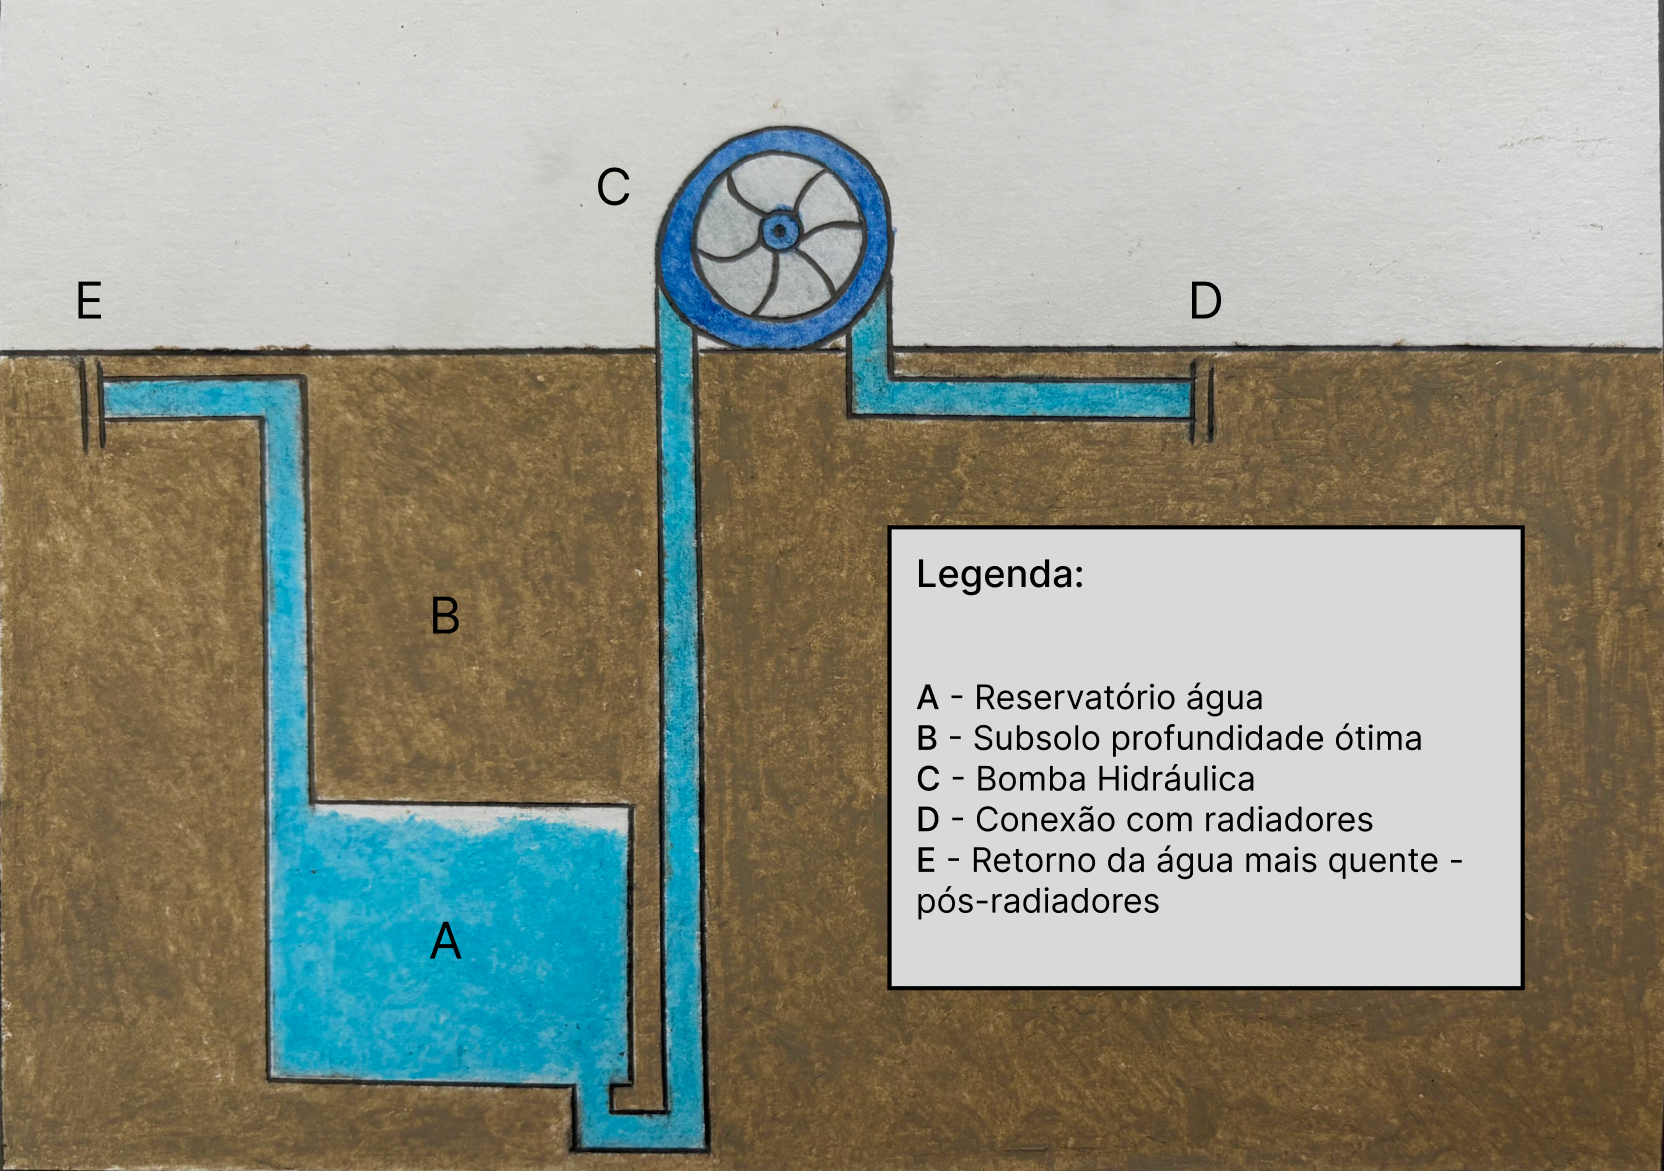
\includegraphics[scale=0.25]{pictures/geoterma.png}
    \caption{Esquema de construção de um poço para refrigeração geotérmica sugerido}
    \label{geothermal-new}
\end{figure}


Essa tecnologia não é benéfica apenas para centros urbanos, pois tem potencial para revolucionar a agricultura. Além de ser possível criar estufas com climatização controlada, é possivel fazer um combate a desertificação com a produção de matéria orgânica e criação de mudas. Portanto, estufas com refrigeração geotérmica atuam no combate à desertificação de múltiplas formas e pode ser a chave para converter terras improdutivas em regiões economicamente autônomas. Porém, para uso em ambientes fechados pode ser necessário o uso de ventiladores atrelados aos radiadores para melhor eficiência em trocas térmicas. Na (\autoref{poste}) exemplifico um uso de radiador ao ar-livre e já na (\autoref{estufa}) é um exemplo para ambiente fechado.

\begin{figure}[ht]
    \centering
    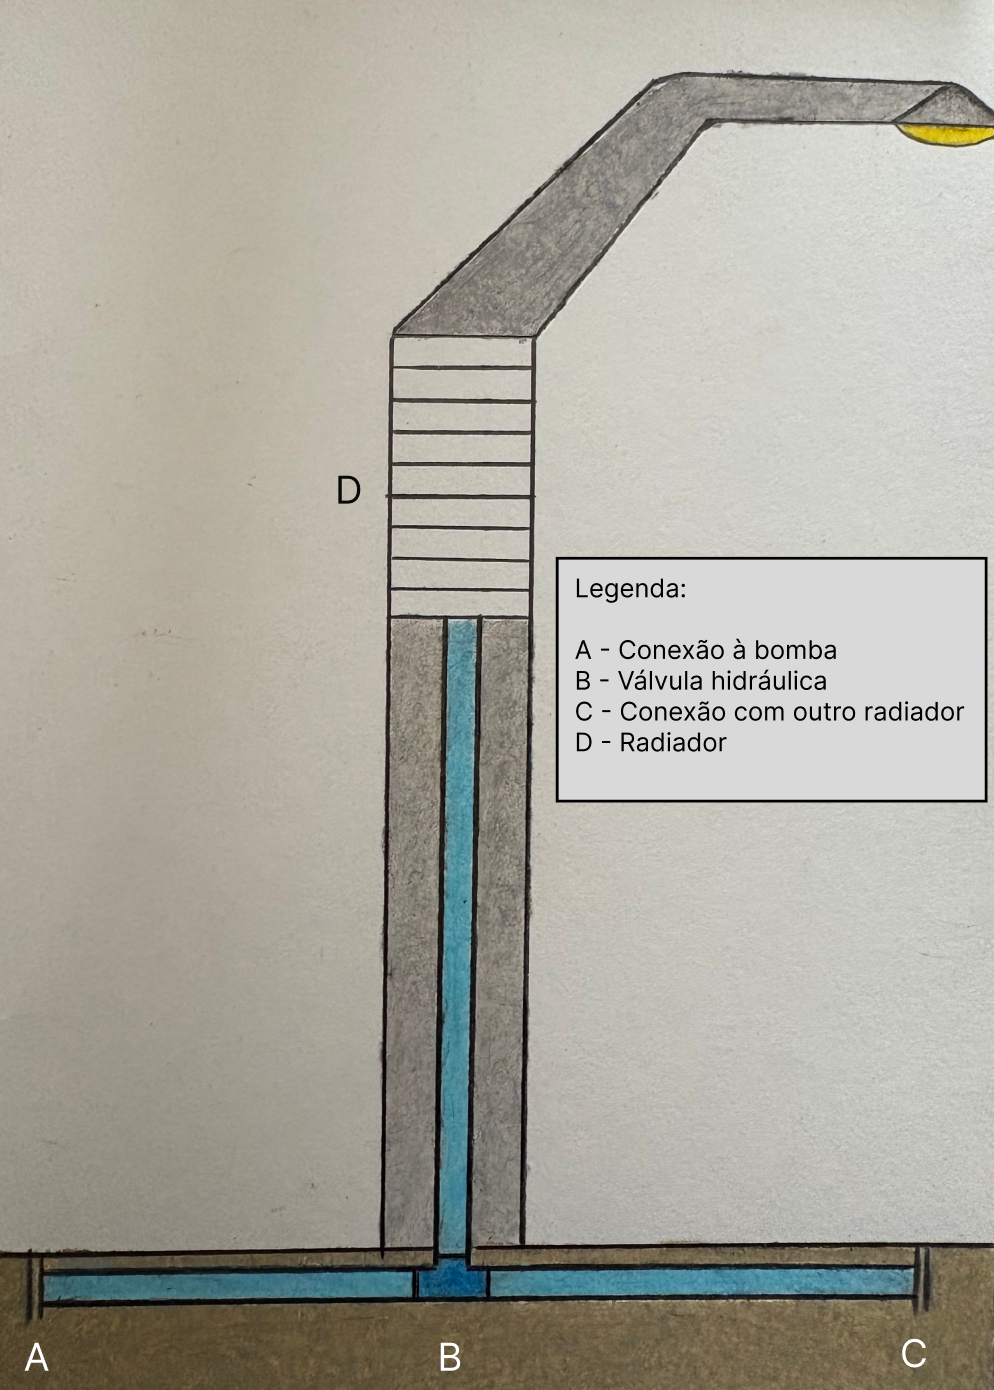
\includegraphics[scale=0.25]{pictures/poste.png}
    \caption{Esquema de construção de um radiador público em um poste}
    \label{poste}
\end{figure}

\begin{figure}[ht]
    \centering
    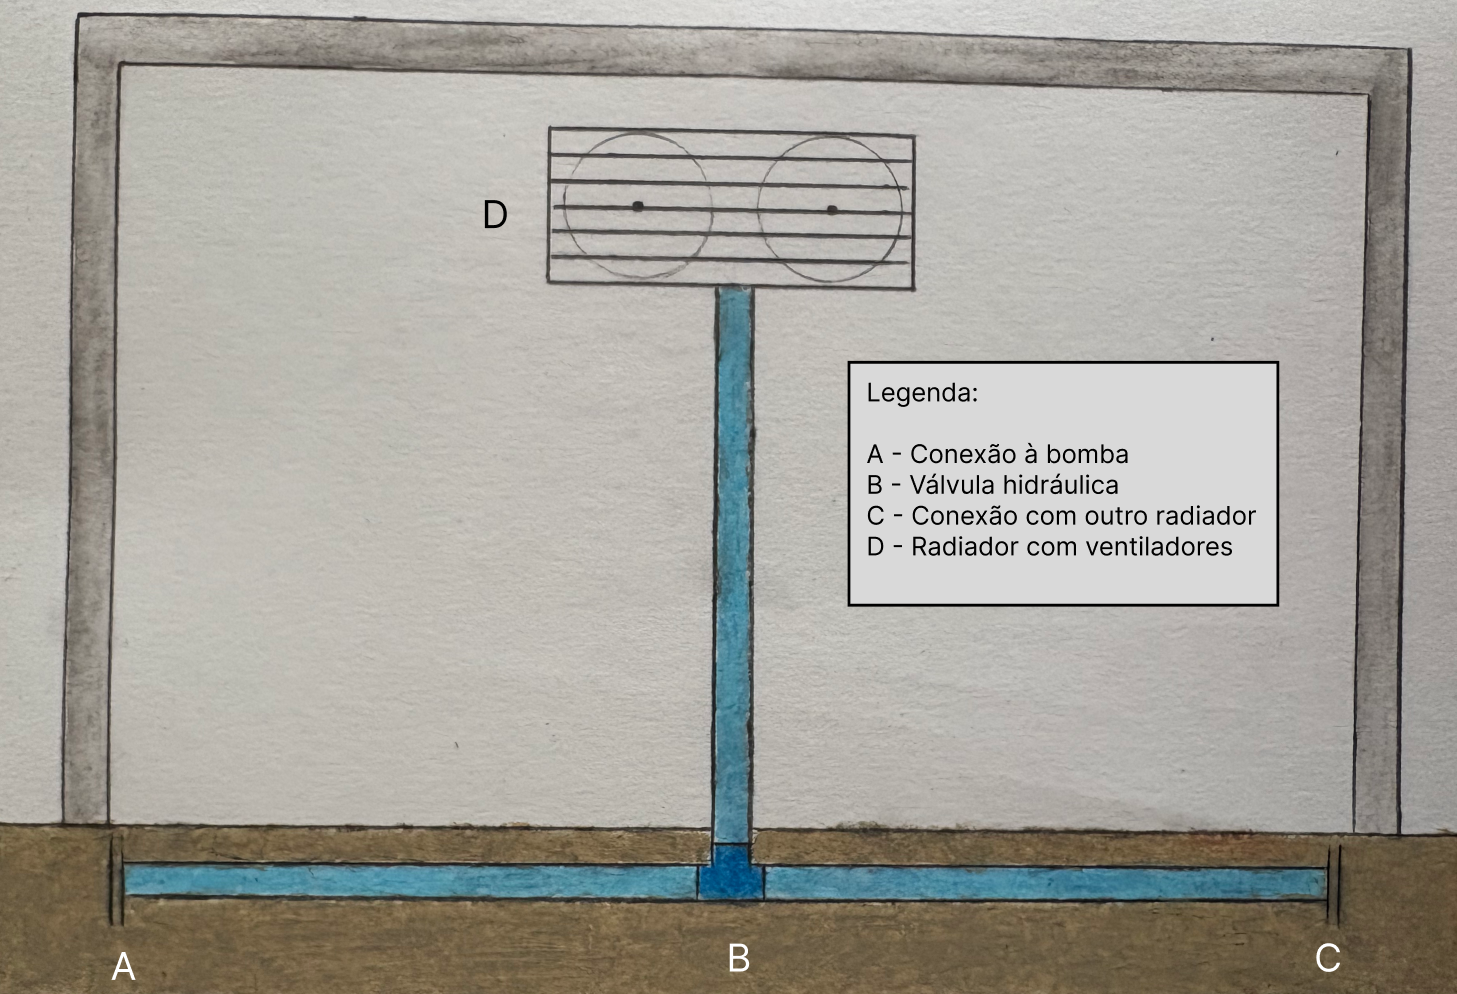
\includegraphics[scale=0.25]{pictures/estufa.png}
    \caption{Esquema de construção de um radiador para ambiente fechado - ex. estufa}
    \label{estufa}
\end{figure}

\section{Experimento}

A tese aqui escrita está em forma puramente teórica e é necessário a criação de um experimento para confirmá-la, deixando sempre bem claro que o desenvolvimento científico deve ser empírico e colaborativo. O experimento proposto é escolher uma região metropolitana com alto uso de ar-condicionados e criar o primeiro refrigerador geotérmico no local. Assim que o refrigerador estiver em funcionamento, é necessário que não se use os ACs e utilize os sistemas de monitoramento meteorológicos para averiguar se o efeito de refrigeração está de acordo com a teoria. Lembrando que ainda não é possível prever quantos sistemas deverão ser construídos para estabilizar a atmosfera terrestre, mesmo se essa teoria estiver válida.

Como já antes mencionado, a temperatura da profundidade ideal para os poços - a qual deve ser em torno de 2m - varia dependendo de diversos fatores como latitude da localização, estação do ano e tipo de solo. Porém, como a quantidade de calor gerada no meio urbano se reduziria com o fim dos ACs, um outro efeito benéfico é que isso seria refletido na temperatura do subsolo com o passar do tempo, ou seja, esse sistema se torna mais eficiente em retirar calor com o passar dos anos.
\chapter[Conclusões]{Conclusões}

A tecnologia de refrigeração geotérmica associada a técnicas mais modernas de agricultura tem o potencial de melhorar o rendimento e qualidade da comida para combater a fome que ainda assola no mundo. E ainda por cima, aplicada nos entornos de regiões desertificadas, pode redirecionar a água proveniente do derretimento das calotas polares para o combate à desertificação. Em resumo, essa tese não apenas deve ser lida como uma esperança contra a Crise climática, mas como o início de uma Revolução Verde no planeta. Se os resultados do experimento aqui descrito forem afirmativos, seria o início de acordos climáticos globais que envolvem a luta contra a fome e contra a desertificação no mundo.

A queima de combustíveis fósseis são essenciais para o funcionamento da sociedade moderna e mesmo que atualmente são considerados a causa das catástofres climáticas, ainda é difícil pensar em uma sociedade sem o seu uso. Essa tese tem como principal objetivo colocar a culpa das mudanças climáticas onde deve, que são nos ar-condicionados, porém, os combustíveis fósseis ainda são uma fonte de energia não renovável e é necessário que a sociedade comece a se planejar para a \textit{Era Pós-Petróleo}.

% ----------------------------------------------------------
% ELEMENTOS PÓS-TEXTUAIS
% ----------------------------------------------------------
\postextual
% ----------------------------------------------------------

% ----------------------------------------------------------
% Referências bibliográficas
% ----------------------------------------------------------
\bibliography{elementos-postextuais/references}

% ----------------------------------------------------------
% Apêndices
% ----------------------------------------------------------
%\input{elementos-postextuais/apendices}

%---------------------------------------------------------------------
% INDICE REMISSIVO
%---------------------------------------------------------------------
\phantompart
\printindex
%---------------------------------------------------------------------

\end{document}